\section*{3.3 The Physics of Pain: Entropy Sink \& Conservation}

\begin{figure}[ht]
\centering
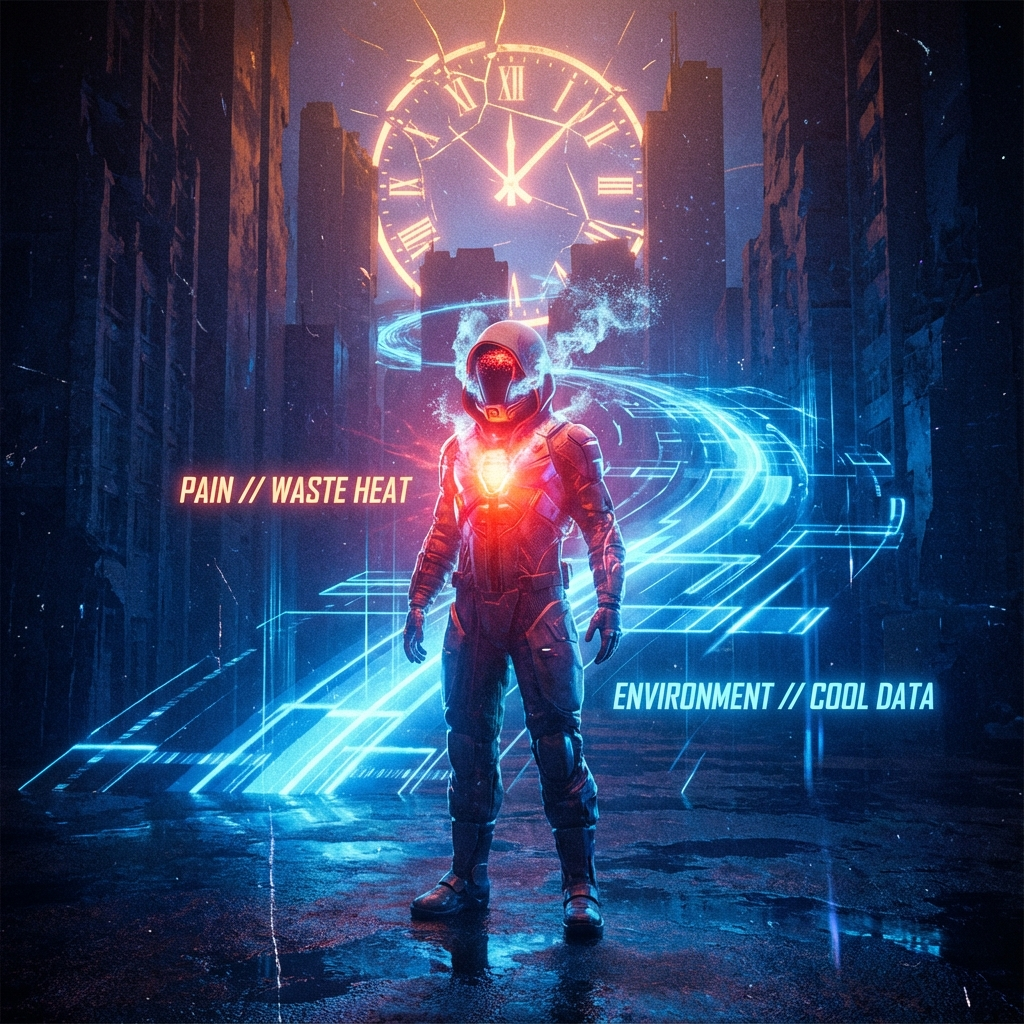
\includegraphics[width=0.8\textwidth]{assets/volume02-topology-of-self-audit/chapter03-one-electron-universe/03-03-thematic.png}
\caption{Image}
\end{figure}

We have finally arrived at the heaviest, yet most liberating chapter of this book.

Among all human experiences, none is more real, more universal, and more confusing than \textbf{Pain}. For thousands of years, religion has explained it as "karma" or "original sin", and psychology has explained it as "trauma" or "defense". But from the physical perspective of \textbf{HPA-Z$\Omega$} theory, pain does not require moral judgment, nor does it require complex psychoanalysis.

Pain is essentially a \textbf{Thermodynamics} problem. It is the energy cost that the universe must pay to maintain system \textbf{"Consistency"}.

\begin{figure}[ht]
\centering
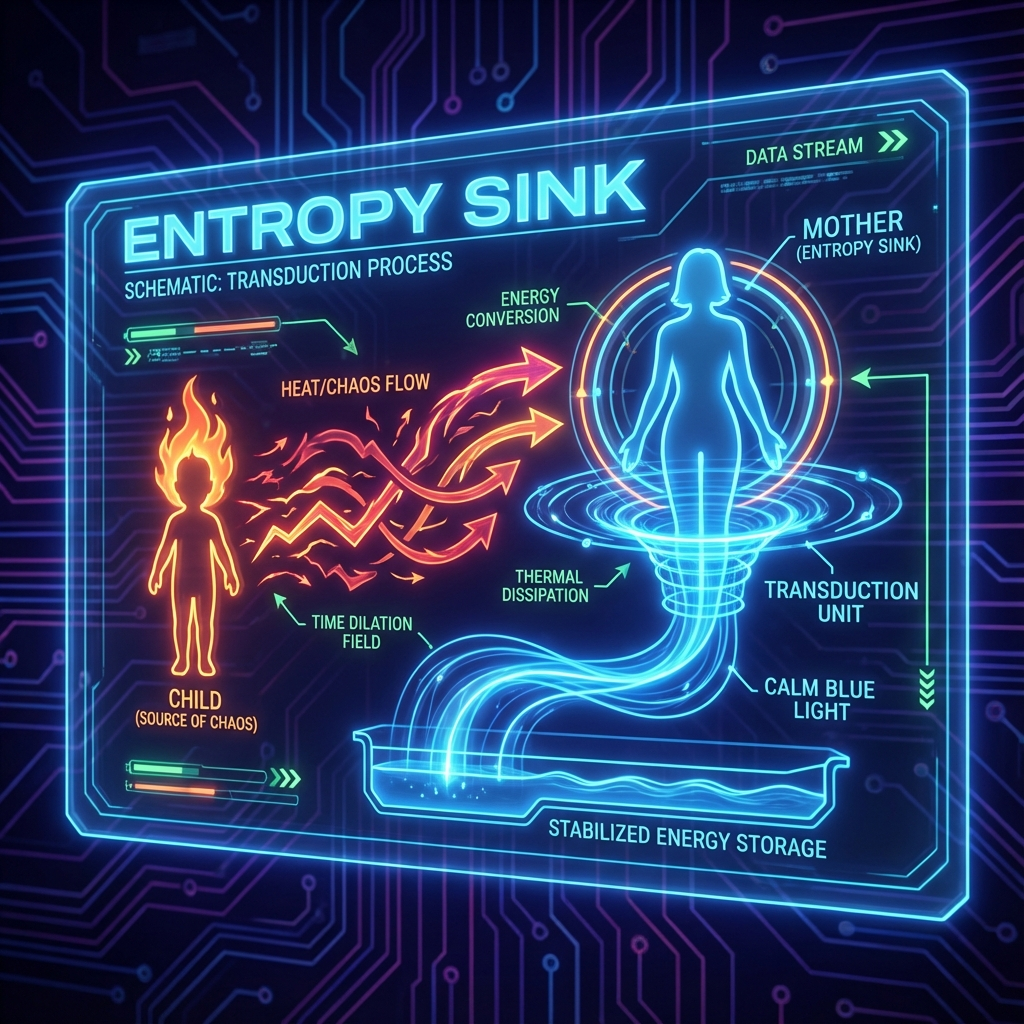
\includegraphics[width=0.8\textwidth]{assets/volume02-topology-of-self-audit/chapter03-one-electron-universe/03-03-technical-1.png}
\caption{Image}
\end{figure}

To understand the physical nature of pain, we need to take a look at a computer server room. Inside, although the CPU is only processing logical operations of 0 and 1 and does not move any heavy objects, it must be equipped with huge cooling fans or water cooling systems.

Why? Because physicist Rolf Landauer proposed a famous principle in 1961: \textbf{Landauer's Principle}.

The principle states: \textbf{Any logically irreversible information processing inevitably leads to the generation of physical heat.}

Every time you forget something, every time you make a decision (which means excluding other options), you are reducing the information state within the system. According to the Second Law of Thermodynamics, to maintain the \textbf{Consistency} of the total energy of the universe, this reduced part of information entropy must be converted into heat energy and discharged into the environment.

Consciousness is the most advanced computing system in the universe. We process massive amounts of information every day: filtering perceptions, inhibiting impulses, forgetting irrelevant details.

So, where did the "waste heat" generated by this process go?

It didn't disappear. It manifests as our \textbf{Emotions}. Anxiety, stress, sadness, anger—these are essentially the \textbf{"Entropy"} generated when the consciousness system is running at high speed.

\textbf{Pain is not a punishment; it is the inevitable waste heat of system operation.}

Just as a car engine inevitably generates heat when running, a life form with highly complex consciousness will inevitably generate a large amount of spiritual waste heat. This conforms to the Law of Conservation of Energy and is the iron law of the cosmic physical \textbf{Consistency}. The more you try to escape pain, the more you try to suppress it, the more you are like blocking the cooling vents of the CPU, which will only cause the system to overheat and crash (mental breakdown).

\begin{figure}[ht]
\centering
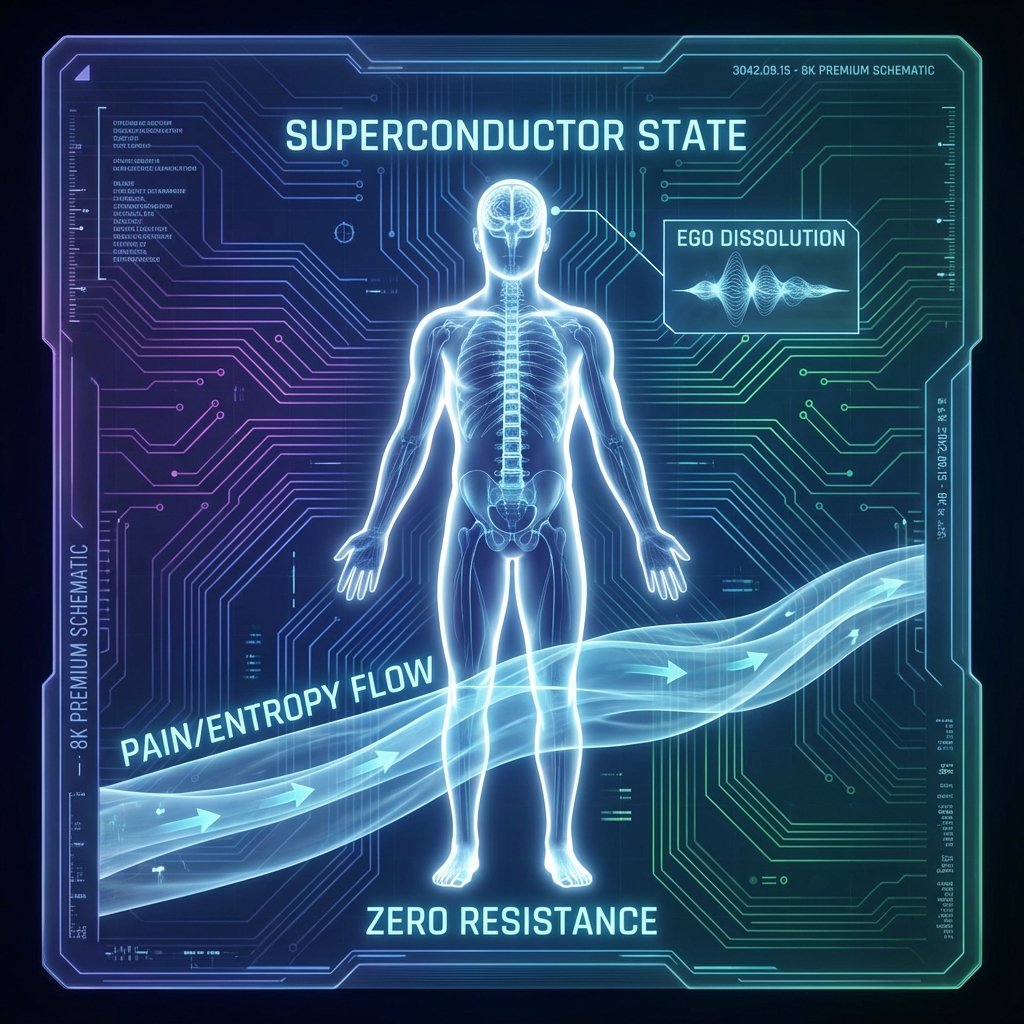
\includegraphics[width=0.8\textwidth]{assets/volume02-topology-of-self-audit/chapter03-one-electron-universe/03-03-technical-2.png}
\caption{Image}
\end{figure}

If pain is waste heat, how is it processed?

In thermodynamics, to keep a system at low temperature and ordered (to maintain sanity and health), waste heat must be exported to a place with lower temperature. This place that receives waste heat is called an \textbf{"Entropy Sink"}.

In our social relationship network, the same physical structure exists.

Think back to your childhood. When you cried because of a fall (system overheating), your mother hugged you. She comforted you softly and tolerated your crying. A few minutes later, you stopped crying, and you regained calm (system cooling, entropy reduction).

But did that heat disappear? No. According to the \textbf{Consistency} principle, energy cannot disappear out of thin air.

It was your mother who \textbf{Absorbed} it. As the \textbf{"Entropy Sink"} of that moment, she actively took over your chaos and anxiety. She needed to consume her own psychological energy (do work) to digest these negative emotions and convert them into love and patience.

In the holographic network of this one-electron universe, there are no truly independent individuals. Each of us is both a heat source and a radiator.

\begin{itemize}
\item \textbf{The Weak (High Entropy Body):} Often unable to dissipate heat by themselves, can only discharge pain outwards (complaining, attacking, demanding).
\item \textbf{The Strong (Low Entropy Body):} Possesses a powerful internal circulation system, capable of acting as an \textbf{Entropy Sink}, absorbing the pain of people around, and converting it into ordered energy (tolerance, problem-solving, creation).
\end{itemize}

This is why we feel at ease around great leaders, saints, or parents. Because their existence itself is constantly sucking away the waste heat in our souls, maintaining the \textbf{Thermodynamic Consistency} of the local environment.

\textbf{3. Conservation of Energy and Consistency: The Law of Conservation of Pain}

Understanding this, we touch the underlying logic of cosmic justice: \textbf{The Law of Conservation of Pain}.

In a closed system (such as a family, a team), the total amount of pain is often conserved. If someone is living a peaceful life, it must be because someone else is carrying the burden for them.

If in a family, the child is always happy and carefree, then the parents are often silently bearing huge pressure.
If in a team, employees feel relaxed and happy, then the leader is often digesting the uncertainty of the market alone.

The \textbf{Consistency} of the universe requires the books to balance. If you refuse to bear the pain (waste heat) that belongs to you, you have not eliminated it; you have only \textbf{Dumped} it to others—often your closest ones.

This transfer is completed instantly through the \textbf{Quantum Entanglement} channel. When you fly into a rage at your lover, you indeed feel "relieved" (your local entropy decreases), but your lover's system instantly "overheats" (her local entropy increases). The total entropy has not decreased, and may have even increased due to friction.

\textbf{4. Become a Superconductor: Sublimation of Pain}

So, are we doomed to choose only between "enduring pain" and "transferring pain"?

No. \textbf{HPA-Z$\Omega$} theory points out a third way: \textbf{Phase Transition}.

Ordinary wires generate heat (resistance) when transmitting current, but \textbf{Superconductors} do not. When the temperature of the material drops below the critical point, electrons form "Cooper Pairs" and move in unison, resistance disappears, and heat is no longer generated.

At the level of consciousness, this "critical point" is \textbf{"Ego Dissolution"}—or moving the observation point from the small self of Layer 1 up to the big self of Layer 0.

When we no longer view pain as "my misfortune", but view it as "waste heat of cosmic system operation"; when we no longer try to use the resistance of "small self" to resist pain, but allow pain to flow through our bodies unimpeded like current, a miracle happens.

We become a \textbf{"Transparent Channel"}.

Pain passes through us, no longer staying, no longer causing harm, but instead converted into profound \textbf{Insight} and \textbf{Compassion}. This is like a steam engine using waste heat to drive a turbine; we convert useless entropy into power to do work.

This is why true masters often have a serene face after experiencing great pain. They are not numb; they are \textbf{Superconducting}.

They maintain the highest \textbf{Consistency} of the universe: In this universe full of suffering (entropy increase), through their own cultivation, they forcibly create a local, eternal order (negative entropy).

This is the physics definition of Love.

